\section{Background} \label{section_background}

The \scps respond to a function of temperature. To precisely control this complicated actuator, an electrical microprocessor was used. Therefore, the methods for electrically operating \scps and investigating their characteristics are discussed.

\subsection{Fabrication of the SCP Artificial Muscles}
The \scps used in this paper were made by twisting silver-painted nylon thread (Conductive Sewing Thread Size 92, Shieldex), which was found to be the best in terms of strain and force production \cite{haines}. First, the conductive thread was piled up four times to make its length be \SI{50}{\centi\meter}. Each side of thread was connected to washers. Then, a wire was hung to one of the washer and a motor to the other. (Figure \ref{silverSCP_2})
As illustrated in figure \ref{silverSCP_illust}, the motor was rotated until the thread created a coil \cite{fab_coil}. After making same one again, two coils were overlapped to each other, making stable form. 
Lastly, they were heated up under an electric current.\footnote{\SI{2.5}{\ampere} was applied and stopped when smoke occurred. While repeating heating and cooling about ten times, the length at ambient temperature got longer and reached at a constant length.} By using this method, \scp was made, which is \SI{10}{\centi\meter} - \SI{11}{\centi\meter} in length and \SI{2.5}{\ohm} in electric resistance at ambient temperature with no external force.

\begin{figure}
	\centering
	\begin{subfigure}{.15\linewidth}
		\centering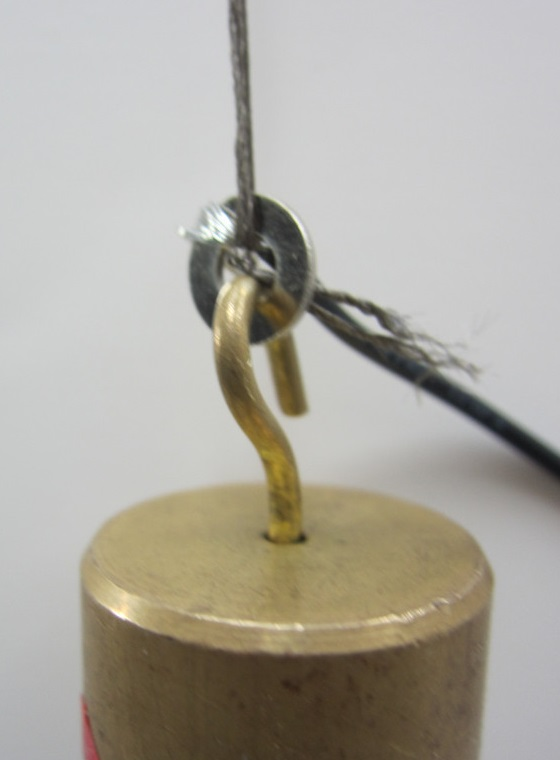
\includegraphics[width=\textwidth]{small_silverSCP_3_v2.jpg}
		\caption{\label{silverSCP_2}}
	\end{subfigure}
	~
	\begin{subfigure}{.45\linewidth}
		\centering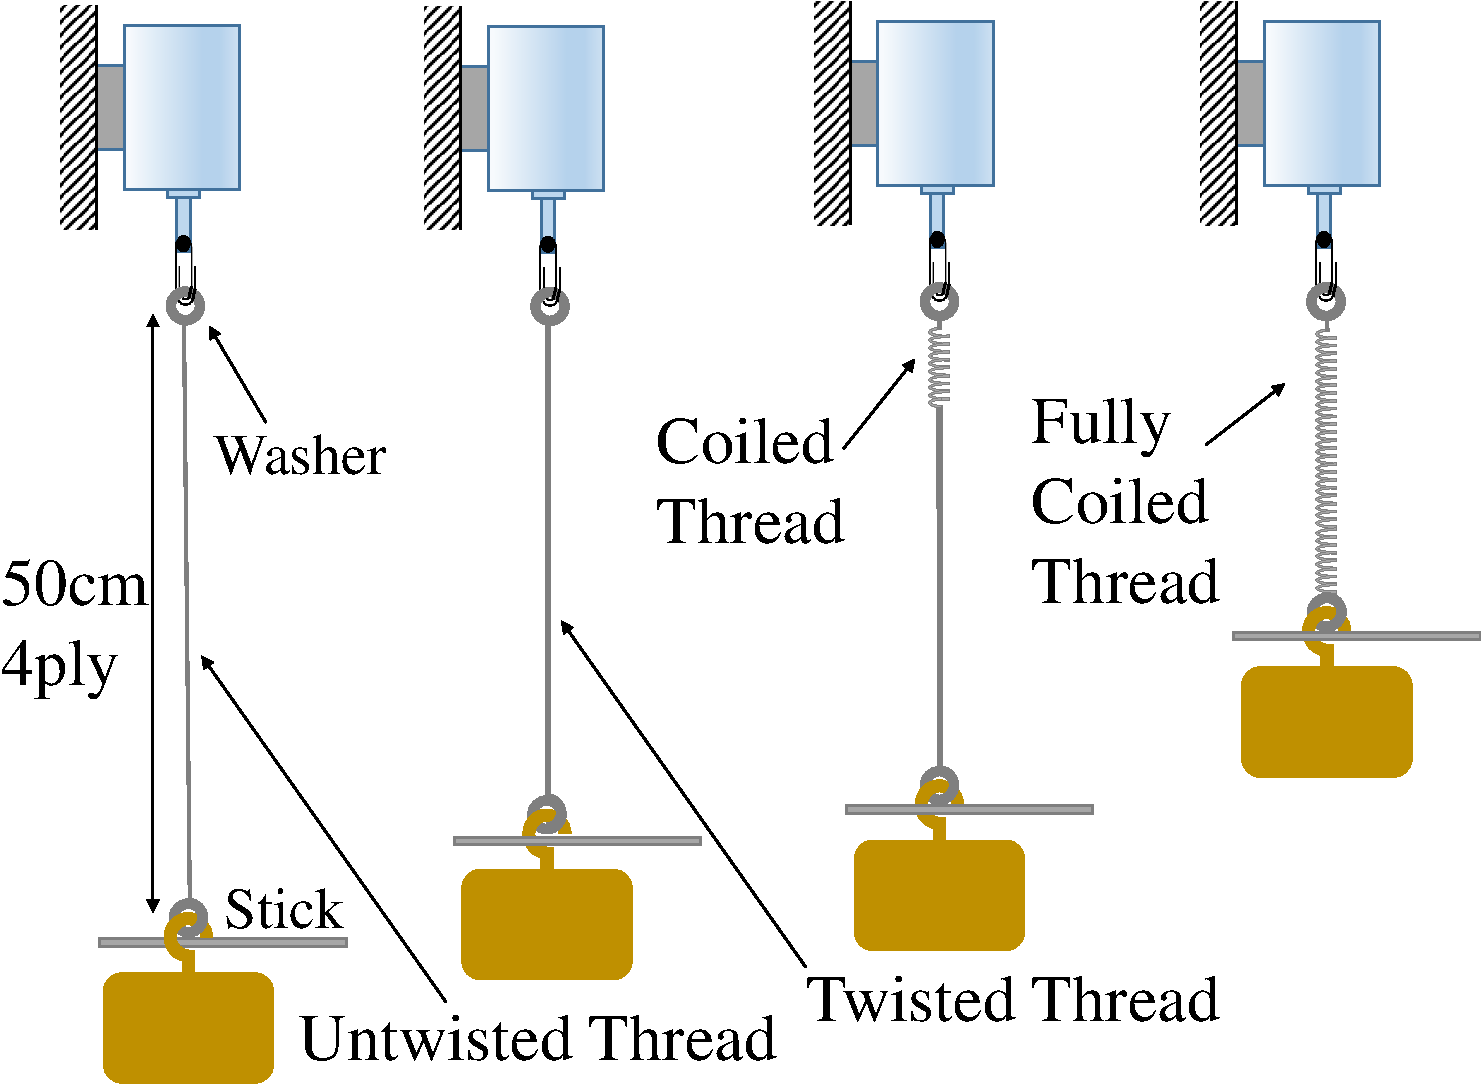
\includegraphics[width=\textwidth]{Fab_illust_v2_crop.pdf}
		\caption{\label{silverSCP_illust}}
	\end{subfigure}
	~
	\begin{subfigure}{.15\linewidth}
		\centering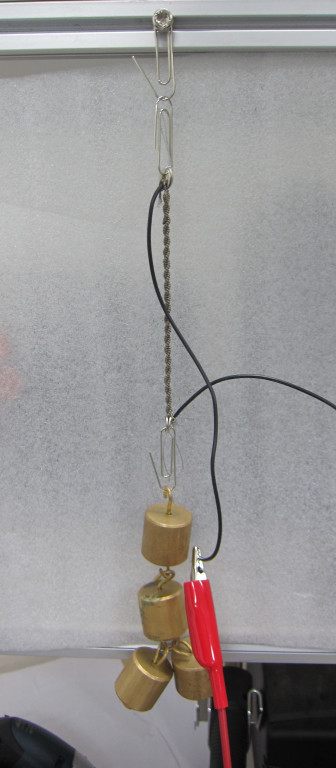
\includegraphics[width=\textwidth]{small_silverSCP_7.jpg}
		\caption{\label{silverSCP_annealing}}
	\end{subfigure}
	\caption[Process of making \scps with silver-painted nylon thread]{\subref{silverSCP_2} 4-ply, \SI{50}{\centi\meter} thread bundle's each side was attached to washers. The upper end was hung on motor, and the lower end was attached to \SI{400}{\gram} weight with a wire inserted in between washer and thread. \subref{silverSCP_illust} To twist a thread until it created a coil, the bottom was fixed with a stick. Then, two super coiled polymers were made. Their upper parts were attached to one clip and their lower parts were hung on \SI{400}{\gram} weight. Coiled thread's thickness was exaggerated. \subref{silverSCP_annealing} By these processes, the \scpnospace, which has wire on its each side, was made. Finally, they were annealed until their length at ambient temperature didn't get longer.}
	\label{silverSCP_makingof}
\end{figure}

\subsection{Actuation of the SCP Artificial Muscles} \label{subsection_actuation}
As discussed in the previous section, the \scp was made with conductive thread in order to electrically control the heat speed. The electrical resistance of the \scp was $R=\SI{2.5}{\ohm}$, so the power $P$ was supplied by applying voltage $V=\sqrt{PR}$. The voltage was controlled by MOSFET and PWM generation of Arduino Uno.

\subsection{\ANTA} \label{subsection_anta}
\scps can be easily heated by applying the electric current. However, cooling demands more sophisticated procedure. Also, muscles can produce force only by contracting, not by relaxing. This means that \scps can't be directly applied to robots which have to produce force in various positions.
Therefore, principle of antagonism was used, which is known to be energy-optimal for various tasks \cite{antagonism}.

